\documentclass[a4paper,10pt]{article}

\usepackage[BoldFont,SlantFont,CJKsetspaces,CJKchecksingle]{xeCJK}
\usepackage{fancyhdr}
\usepackage{amsmath}
\usepackage{amssymb}
\usepackage{amsthm}
\usepackage{multirow}
\usepackage{longtable}
\usepackage{graphicx}
\usepackage{xcolor}
\usepackage{float}
\usepackage{tikz,pgfplots}
\usepackage{pifont}
\usetikzlibrary{arrows,scopes,svg.path,shapes,shadows,positioning,decorations.markings}
\usepackage{verbatim}
\usepackage[colorlinks,linkcolor=black,anchorcolor=blue,citecolor=green,filecolor=blue,urlcolor=blue]{hyperref}
\usepackage{listings}
\usepackage{setspace}
\usepackage{indentfirst}
\usepackage{cleveref}
\usepackage{mathrsfs}

\parindent 2em

\setCJKmainfont[BoldFont=SimHei,ItalicFont=KaiTi_GB2312]{SimSun}
\setCJKmonofont{SimSun}

\newtheorem{lemma}{\textbf{引理}}
\newtheorem{theorem}{\textbf{定理}}


\title{Sudoku Game Report}

\author{计64~~陶东来~~~学号:2016011322}

\begin{document}
    \maketitle
    \section{概述}

    本次大作业,我本来想使用传统的Qt来完成。但我在实现过程中发现,我难以简洁地达成我想要的效果。并且,Qt的QSS并不像CSS那样有
    方便的工具(jQuery)来辅助处理。因此我选择转换思路,把工程分解成了由html+css+js管理的前端,和用Qt管理的后端,通过QWebEngine和
    QWebChannel来进行前后端的交互。

    必须说明的是,本次所实现的版本仅仅是一个“原型”。更多的视觉效果,如动画,可以在前端中较为方便地扩展出来(使用keyframe),比起单纯
    的Qt要简单得多。这也是我使用这种设计的重要原因之一。

    \section{前端}

    前端使用了jQuery和bootstrap来辅助实现,通过js来管理游戏的整体运行时逻辑。运行效果如图1:

    \begin{figure}
        \centering
        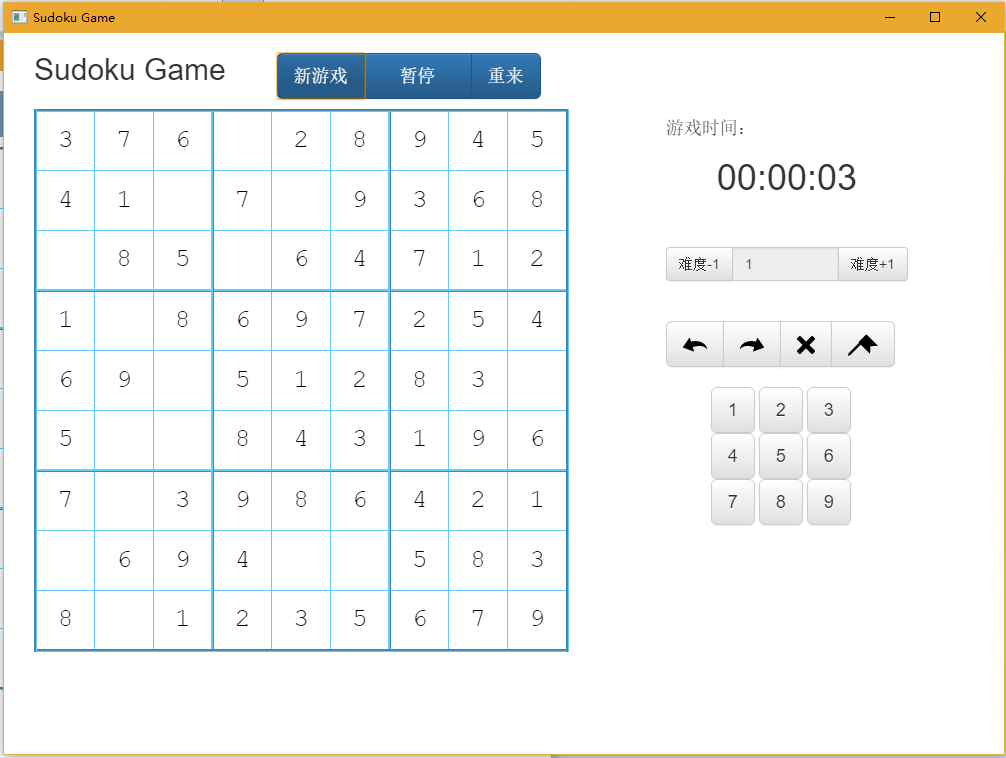
\includegraphics[height=5cm]{new_game_lvl1.png}
        \caption{图1. 难度为1}
    \end{figure}

    可以调节难度,在难度为10时,效果如图2:

    \begin{figure}
        \centering
        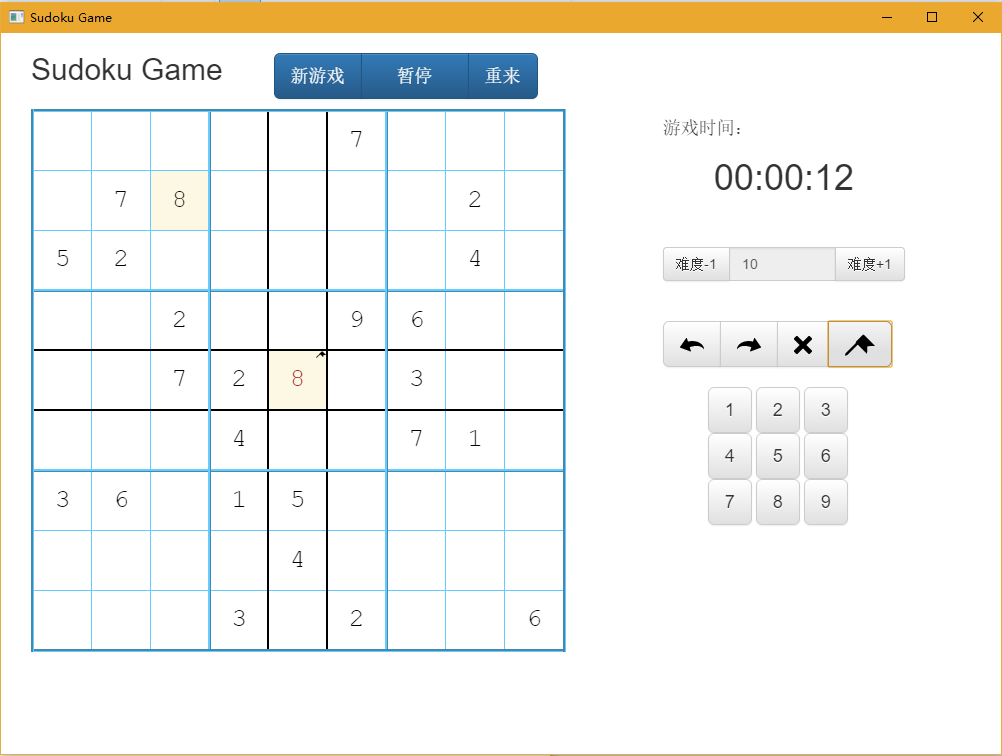
\includegraphics[height=5cm]{playing_lvl10.png}
        \caption{图2. 难度为10}
    \end{figure}

    可以看到,支持了相同数字高亮,标记格子,提示当前行列的功能。
    而一行中填入多个数字,计时,撤销,恢复,删除,重新开始,这些功能这些功能也不在话下。

    \begin{figure}
        \centering
        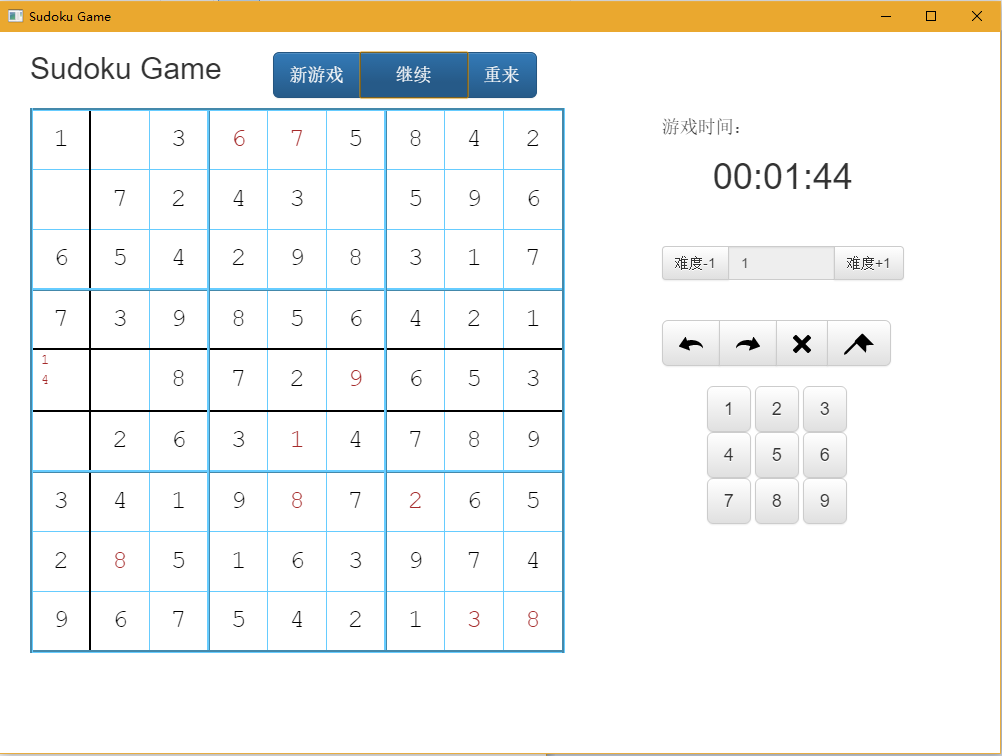
\includegraphics[height=5cm]{playing_lvl1.png}
        \caption{图3. 一行中填入多个数字}
    \end{figure}

    最后,是一张游戏胜利的截图。

    \begin{figure}
        \centering
        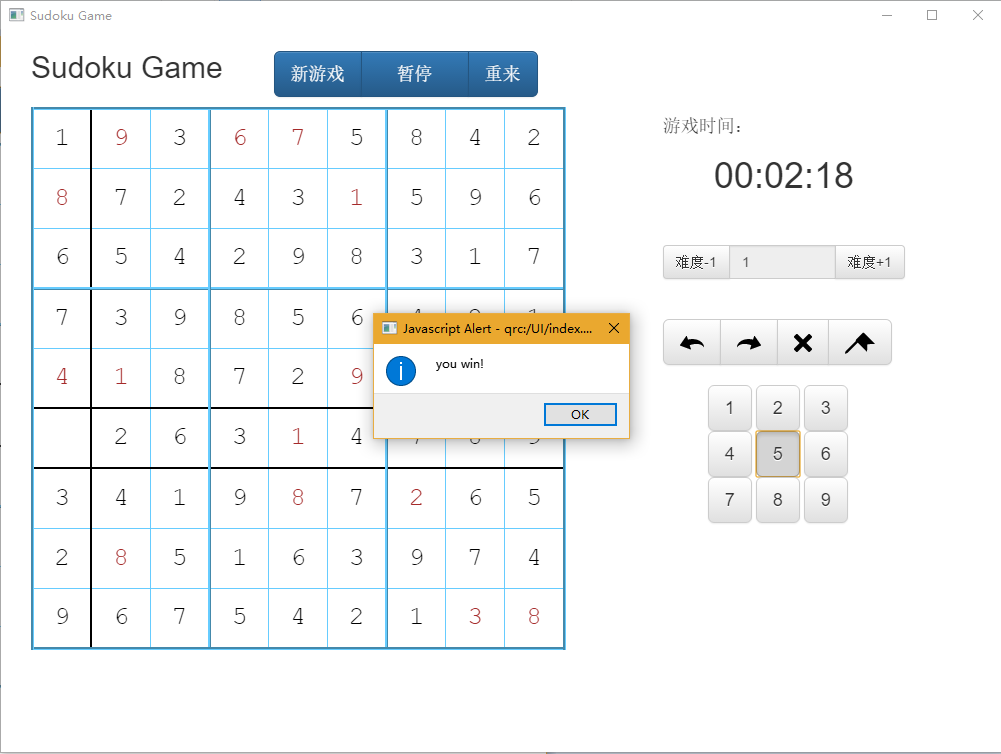
\includegraphics[height=5cm]{win_lvl1.png}
        \caption{图4. 胜利!}
    \end{figure}
    \section{后端}

    后端的Qt主要负责数独盘面的产生,并通过QWebChannel传输至前端。并且,通过Qt后端,游戏进度的保存也成为可能。

    \section{数独的求解及生成}

    数独的求解使用了经典的DLX(Dancing Link X)算法。数独的生成则参考了同学交流时所提到的Las Vegas+贪心挖洞算法。
    而难度则直观地表现在盘面空格的个数上。难度大于等于$x$时,盘面上的空格数应至少为$10+5x$个。

        \subsection{数独的求解——DLX}

        DLX算法是由Donald Knuth提出的,用以高效解决精确覆盖问题的搜索算法。所谓精确覆盖问题的一个表述是,给定一个01矩阵,
        求得一个行的集合,使得每列有且仅有一个1,或报告无解。

        首先,我们不难想到一个深度优先搜索算法(被Knuth称为算法X)。从第一列开始,对于第i列,我们依次考虑当下可以用来覆盖这一列
        的行,并把之后将与之冲突的所有行排除在之后的考虑范围之内,接着考虑第i+1列。为了高效地实现算法X,我们可以使用二维的循环双向
        链表来存储这个01矩阵,这个链表就被称作Dancing Links。通过Dancing Links,我们可以高效地删除/恢复行列,并且更好地利用
        稀疏矩阵的特性,从而获得极佳的速度。

        DLX的具体实现这里不进行细致的描述。我们主要要谈的是如何将数独转化为精确覆盖问题。我们构造一个$9 \times 9 \times 9$行,
        $4 \times 9 \times 9$列的矩阵。行表示在格子$(i,j)$中填入$k$,而列表示其对应的4条限制:
        \begin{enumerate}
            \item $(i,j)$有且仅有一个数字。
            \item 数独的第$i$行有且仅有一个数字$k$。
            \item 第$j$行有且仅有一个数字$k$。
            \item $(i,j)$所在的$3 \times 3$大方格有且仅有一个数字$k$。
        \end{enumerate}

        转化完毕之后,直接使用DLX算法求解即可。

        \subsection{数独的生成——Las Vegas+贪心挖洞}

        数独的生成分为两步:1.生成一个合法的终盘;2.在终盘上挖出一些空格。

        \subsubsection{生成合法终盘——Las Vegas}

        一个简单易行的方法,是在全空数独上随机地选取MN个格子,随机填入1-9的数字,在调用数独求解器得到终盘,如果无解则重新
        随机。这里根据实践,MN取11。

        \subsubsection{挖洞——贪心法}

        在获得了一个合法的终盘之后,我们根据难度选择对应的遍历方法$g_i$,并对遍历过程中的每个格子,尝试将其变为空格。如果
        在变为空格之后盘面有唯一解,就保留这个空格,否则将其恢复为原来的数字。重复这个过程知道空格数达到难度要求为止。

        具体实现时,考虑到不同的遍历方法$g_i$,实际上只是遍历顺序有区别,而对于遍历的每个格子实际上做的是同样的事情,我使用
        了FP的思想,让$g_i$接受一个function作为参数,这个function执行了对于单个格子进行的操作,如图5。

        \begin{figure}
            \centering
            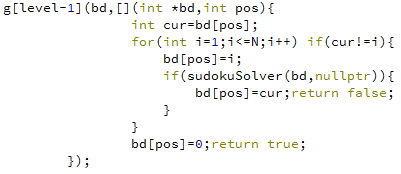
\includegraphics{generator.png}
            \caption{图5. 实现}
        \end{figure}
    \section{值得加入的改进}

    通过加入动画让UI更为炫酷;

    保存最佳成绩;

    等等。

    \section{吐槽}

    等等,还有吐槽环节吗?第二周怎么还是Qt?真是个灾难!

    话说回来,我这次的UI是基于高二的一个(尚未完成的)project的(半成品)web\_ui,现在还挂在github上面
    (https://github.com/NagiNikaido/Cell-Game)。真是久违了啊,在我想起它的时候,有一种“啊,兜兜转转又回到了这里”的感觉。
    我刚开始写这个project的时候,想着能不能搞个arena,让AI无监督自进化。再后来为了可视化,参考当时正火的2048开始用bootstrap来
    做web\_ui,服务器还打算用node.js来写。再后来,就因为种种原因被搁置起来了。

    或许什么时候我又会把它拿出来,精心擦拭一番,换上新的零部件,加上全新的扩展——特修斯之船。

    不过,那应该也是以后的事情了吧。
\end{document}
